\chapter{Expresiones Regulares y Análisis Léxico en JavaScript}

% Power Sh. JavaScript Cookbook. Chapter 1. Working with JavaScript Strings
% David Flanagan. JavaScript, the Definitive Guide. O'Reilly.  Chapter 10.
% JavaScript. The Missing Manual. Chapter 4. working with words, numbers and dates. A quick object lesson

\section{Mozilla Developer Network: Documentación}

\begin{enumerate}
\item \htmladdnormallink{RegExp Objects}{https://developer.mozilla.org/en-US/docs/JavaScript/Reference/Global_Objects/Regexp}
\item 
\htmladdnormallink{exec}{https://developer.mozilla.org/en-US/docs/JavaScript/Reference/Global_Objects/RegExp/exec}
\item 
\htmladdnormallink{search}{https://developer.mozilla.org/en-US/docs/JavaScript/Reference/Global_Objects/String/search}
\item 
\htmladdnormallink{match}{https://developer.mozilla.org/en-US/docs/JavaScript/Reference/Global_Objects/String/match}
\item 
\htmladdnormallink{replace}{https://developer.mozilla.org/en-US/docs/JavaScript/Reference/Global_Objects/String/replace}
\end{enumerate}

\sectionpractica{Conversor de Temperaturas}

\parrafo{index.html}
\begin{verbatim}
<html>
  <head>
      <meta http-equiv="Content-Type" content="text/html; charset=UTF-8">
      <title>JavaScript Temperature Converter</title>
      <link href="global.css" rel="stylesheet" type="text/css">

     <script type="text/javascript" src="temperature.js"></script>
  </head>
  <body>
    <h1>Temperature Converter</h1>
    <table>
      <tr>
        <th>Enter  Temperature (examples: 32F, 45C, -2.5f):</th>
        <td><input id="original" onchange="calculate();"></td>
      </tr>
      <tr>
        <th>Converted Temperature:</th>
        <td><span class="output" id="converted"></span></td>
      </tr>
    </table>
  </body>
</html>
\end{verbatim}

\begin{verbatim}
th, td      { vertical-align: top; text-align: right; font-size:large; }     
#converted  { color: red; font-weight: bold; font-size:large;          }    
input       { text-align: right;  border: none; font-size:large;       }   
body
{
 background-color:#b0c4de;  /* blue */
 font-size:large;
}
\end{verbatim}

\begin{verbatim}
"use strict"; // Use ECMAScript 5 strict mode in browsers that support it
function calculate() {
  var result;
  var original       = document.getElementById("........");
  var temp = original.value;
  var regexp = /.............................../;
  
  var m = temp.match(......);
  
  if (m) {
    var num = ....;
    var type = ....;
    num = parseFloat(num);
    if (type == 'c' || type == 'C') {
      result = (num * 9/5)+32;
      result = ..............................
    }
    else {
      result = (num - 32)*5/9;
      result = ............................
    }
    converted.innerHTML = result;
  }
  else {
    converted.innerHTML = "ERROR! Try something like '-4.2C' instead";
  }
}
\end{verbatim}

\sectionpractica{Comma Separated Values}

\parrafo{Introducción al formato CSV}

Véase \wikip{Comma Separated Values}{Comma-separated_values} en la Wikipedia:

{\it A comma-separated values (CSV) file stores tabular data (numbers
and text) in plain-text form. 
 A CSV file consists of any number of
records, separated by line breaks of some kind; each record consists
of fields, separated by a comma. All records have an identical
sequence of fields.}

\parrafo{Ejemplo de ejecución}

\begin{figure}[htb]
\begin{center}
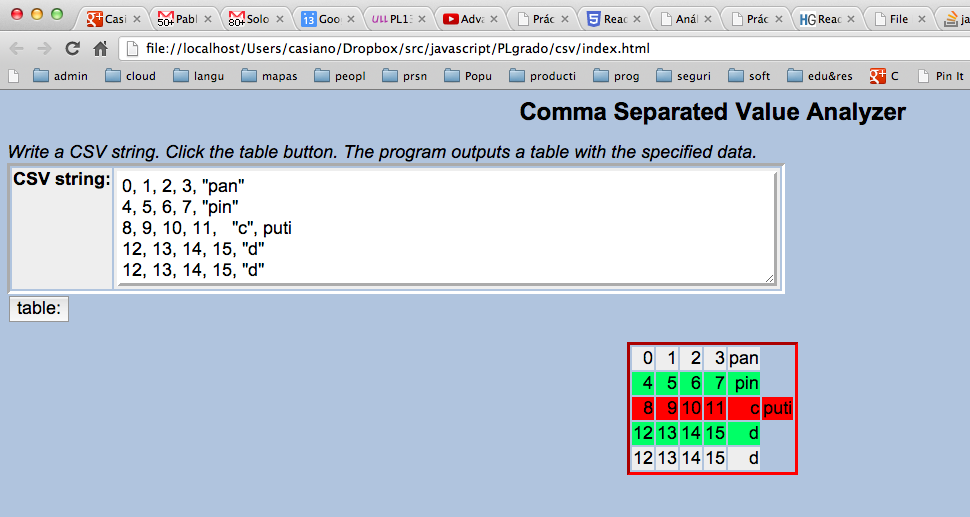
\includegraphics[scale=0.5]{chapter2/csv.png}
\end{center}
\label{figure:csv}
\caption{Ejemplo de pantalla de La aplicación para el Análisis de Datos en Formato CSV}
\end{figure}

\parrafo{Aproximación al análisis mediante expresiones regulares de CSV}
Una primera aproximación sería hacer \verb|split| por las comas:
\begin{verbatim}
> x = '"earth",1,"moon",9.374'
'"earth",1,"moon",9.374'
> y = x.split(/,/)
[ '"earth"', '1', '"moon"', '9.374' ]
\end{verbatim}

Esta solución deja las comillas dobles en los campos entrecomillados. 
Peor aún, los campos entrecomillados pueden contener comas, en cuyo 
caso la división proporcionada por \verb|split| sería errónea:
\begin{verbatim}
> x = '"earth, mars",1,"moon, fobos",9.374'
'"earth, mars",1,"moon, fobos",9.374'
> y = x.split(/,/)
[ '"earth', ' mars"', '1', '"moon', ' fobos"', '9.374' ]
\end{verbatim}

La siguiente expresión regular reconoce cadenas de comillas dobles
con secuencias de escape seguidas opcionalmente de una coma:
\begin{verbatim}
> x = '"earth, mars",1,"moon, fobos",9.374'
'"earth, mars",1,"moon, fobos",9.374'
> r = /"((?:[^"\\]|\\.)*)"\s*,?/g
/"((?:[^"\\]|\\.)*)"\s*,?/g
> w = x.match(r)
[ '"earth, mars",', '"moon, fobos",' ]
\end{verbatim}

Esta otra expresión regular \verb#/([^,]+),?|\s*,/# actúa de forma parecida al \verb|split|. 
Reconoce secuencias no vacías de caracteres que no contienen comas seguidas opcionalmente
de una coma o bien una sóla coma (precedida opcionalmente de blancos):
\begin{verbatim}
> x = '"earth, mars",1,"moon, fobos",9.374'
'"earth, mars",1,"moon, fobos",9.374'
> r = /([^,]+),?|\s*,/g
/([^,]+),?|\s*,/g
> w = x.match(r)
[ '"earth,', ' mars",', '1,', '"moon,', ' fobos",', '9.374' ]
\end{verbatim}

\parrafo{index.html}
\begin{verbatim}
<html>
  <head>
     <meta http-equiv="Content-Type" content="text/html; charset=UTF-8">
     <title>CSV Analyzer</title>
     <link href="global.css" rel="stylesheet" type="text/css">

     <script type="text/javascript" src="../../underscore/underscore.js"></script>
     <script type="text/javascript" src="../../jquery/starterkit/jquery.js"></script>
     <script type="text/javascript" src="csv.js"></script>
  </head>
  <body>
    <h1>Comma Separated Value Analyzer</h1>
    <div>
      <i>Write a CSV string. Click the table button. The program outputs a table with the specified data.</i>
    </div>
    <table>
      <tr>
        <th>CSV string:</th> <!-- autofocus attribute is HTML5 -->
        <td><textarea autofocus cols = "80" rows = "5" id="original"></textarea></td> 
      </tr>
    </table>
    <button type="button">table:</button><br>
    <span class="output" id="finaltable"></span>
  </body>
</html>
\end{verbatim}

\begin{enumerate}
\item 
\htmladdnormallink{jQuery}{http://jquery.com/} (\htmladdnormallink{Descarga la librería}{http://jquery.com/download/})
\item \htmladdnormallink{Underscore}{http://underscorejs.org/}
\item 
\htmladdnormallink{autofocus}{http://www.w3api.com/wiki/HTML5:INPUT.autofocus}.
Véase también \cite{pilgrimhtml5}
\item \htmladdnormallink{textarea}{http://www.w3schools.com/tags/tag_textarea.asp}
\item \htmladdnormallink{button}{http://www.w3schools.com/tags/tag_button.asp}
\end{enumerate}

\parrafo{global.css}
\begin{verbatim}
html *
{
   font-size: large; 
   /* The !important ensures that nothing can override what you've set in this style (unless it is also important). */
   font-family: Arial;
}

h1            { text-align: center; font-size: x-large; }
th, td        { vertical-align: top; text-align: right; }   
/* #finaltable  * { color: white; background-color: black; }   */

/* #finaltable table { border-collapse:collapse; } */
/* #finaltable table, td { border:1px solid white; } */
#finaltable:hover td { background-color: blue; } 
tr:nth-child(odd)    { background-color:#eee; }
tr:nth-child(even)    { background-color:#00FF66; }
input        { text-align: right;  border: none;       }     /* Align input to the right  */
textarea     { border: outset; border-color: white;       }                        
table        { border: inset; border-color: white; }
table.center { margin-left:auto; margin-right:auto; }
#result      { border-color: red; }
tr.error       { background-color: red; }
body
{
 background-color:#b0c4de;  /* blue */
}
\end{verbatim}

\begin{enumerate}
\item 
\htmladdnormallink{Introducción a las pseudo clases de CSS3}{http://www.genbetadev.com/desarrollo-web/introduccion-a-las-pseudo-clases-de-css3}
\item 
\htmladdnormallink{CSS pattern matching}{http://www.w3.org/TR/CSS2/selector.html\#pattern-matching}
\item 
\htmladdnormallink{CSS class selectors}{http://www.w3.org/TR/CSS2/selector.html\#class-html}
\item 
\htmladdnormallink{CSS3: nth-child() selector}{http://www.w3schools.com/cssref/sel_nth-child.asp}
\item 
\htmladdnormallink{CSS: border}{http://www.tizag.com/cssT/border.php}
\item 
\end{enumerate}


\parrafo{csv.js}

\begin{verbatim}
// See http://en.wikipedia.org/wiki/Comma-separated_values
"use strict"; // Use ECMAScript 5 strict mode in browsers that support it

$(document).ready(function() {
   $("button").click(function() {
     calculate();
   });
 });

function calculate() {
  var result;
  var original       = document.getElementById("original");
  var temp = original.value;
  var regexp = /_____________________________________________/g;
  var lines = temp.split(/\n+\s*/);
  var commonLength = NaN;
  var r = [];
  // Template using underscore
  var row = "<% _.each(items, function(name) { %>"     +
            "                    <td><%= name %></td>" +
            "              <% }); %>";

  if (window.localStorage) localStorage.original  = temp;
  
  for(var t in lines) {
    var temp = lines[t];
    var m = temp.match(regexp);
    var result = [];
    var error = false;
    
    if (m) {
      if (commonLength && (commonLength != m.length)) {
        //alert('ERROR! row <'+temp+'> has '+m.length+' items!');
        error = true;
      }
      else {
        commonLength = m.length;
        error = false;
      }
      for(var i in m) {
        var removecomma = m[i].replace(/,\s*$/,'');
        var remove1stquote = removecomma.replace(/^\s*"/,'');
        var removelastquote = remove1stquote.replace(/"\s*$/,'');
        var removeescapedquotes = removelastquote.replace(/\\"/,'"');
        result.push(removeescapedquotes);
      }
      var tr = error? '<tr class="error">' : '<tr>';
      r.push(tr+_.template(row, {items : result})+"</tr>");
    }
    else {
      alert('ERROR! row '+temp+' does not look as legal CSV');
      error = true;
    }
  }
  r.unshift('<p>\n<table class="center" id="result">');
  r.push('</table>');
  //alert(r.join('\n')); // debug
  finaltable.innerHTML = r.join('\n');
}

window.onload = function() {
  // If the browser supports localStorage and we have some stored data
  if (window.localStorage && localStorage.original) {
    document.getElementById("original").value = localStorage.original;
  }
};
\end{verbatim}

\begin{enumerate}
\item 
\htmladdnormallink{Tutorials:Getting Started with jQuery}{http://docs.jquery.com/Tutorials:Getting_Started_with_jQuery}
\item 
\htmladdnormallink{Underscore: template}{http://underscorejs.org/\#template}
\item 
\htmladdnormallink{Stackoverflow::how to use Underscore template}{http://stackoverflow.com/questions/4778881/how-to-use-underscore-js-as-a-template-engine}
\item 
\htmladdnormallink{Como usar localstorage}{http://html5facil.com/tutoriales/como-usar-local-storage-de-javascript}
\item 
\htmladdnormallink{HTML5 Web Storage}{http://www.w3schools.com/html/html5_webstorage.asp}
\end{enumerate}



\section{Ejercicios}

\begin{enumerate}
\item  Paréntesis:
\begin{verbatim}
> str = "John Smith"
'John Smith'
> newstr = str.replace(re, "$2, $1")
'Smith, John'
\end{verbatim}
\item  El método \verb|exec|.

If your regular expression uses the \verb"g" flag, you can use the \verb|exec|
method multiple times to find successive matches in the same string.
When you do so, the search starts at the substring of str specified
by the regular expression's \verb|lastIndex| property.

\begin{verbatim}
> re = /d(b+)(d)/ig
/d(b+)(d)/gi
> z = "dBdxdbbdzdbd"
'dBdxdbbdzdbd'
> result = re.exec(z)
[ 'dBd', 'B', 'd', index: 0, input: 'dBdxdbbdzdbd' ]
> re.lastIndex
3
> result = re.exec(z)
[ 'dbbd', 'bb', 'd', index: 4, input: 'dBdxdbbdzdbd' ]
> re.lastIndex
8
> result = re.exec(z)
[ 'dbd', 'b', 'd', index: 9, input: 'dBdxdbbdzdbd' ]
> re.lastIndex
12
> z.length
12
> result = re.exec(z)
null
\end{verbatim}
\item JavaScript tiene lookaheads:
\begin{verbatim}
> x = "hello"
'hello'
> r = /l(?=o)/
/l(?=o)/
> z = r.exec(x)
[ 'l', index: 3, input: 'hello' ]
\end{verbatim}
\item JavaScript no tiene lookbehinds:
\begin{verbatim}
> x = "hello"
'hello'
> r = /(?<=l)l/
SyntaxError: Invalid regular expression: /(?<=l)l/: Invalid group
> .exit
\end{verbatim}
\begin{verbatim}
[~/Dropbox/src/javascript/PLgrado/csv(master)]$ irb
ruby-1.9.2-head :001 > x = "hello"
 => "hello" 
ruby-1.9.2-head :002 > r = /(?<=l)l/
 => ll 
ruby-1.9.2-head :008 > x =~ r
 => 3 
ruby-1.9.2-head :009 > $&
 => "l" 
\end{verbatim}
\item 
El siguiente ejemplo comprueba la validez de números de teléfono:
\begin{verbatim}
$ cat phone.html 
<!DOCTYPE html>
<html>  
  <head>  
    <meta http-equiv="Content-Type" content="text/html; charset=ISO-8859-1">  
    <meta http-equiv="Content-Script-Type" content="text/javascript">  
    <script type="text/javascript">  
      var re = /\(?\d{3}\)?([-\/\.])\d{3}\1\d{4}/;  
      function testInfo(phoneInput){  
        var OK = re.exec(phoneInput.value);  
        if (!OK)  
          window.alert(RegExp.input + " isn't a phone number with area code!");  
        else
          window.alert("Thanks, your phone number is " + OK[0]);  
      }  
    </script>  
  </head>  
  <body>  
    <p>Enter your phone number (with area code) and then click "Check".
        <br>The expected format is like ###-###-####.</p>
    <form action="#">  
      <input id="phone"><button onclick="testInfo(document.getElementById('phone'));">Check</button>
    </form>  
  </body>  
</html>
\end{verbatim}
\item 
¿Con que cadenas casa  la expresión regular \verb|/^(11+)\1+$/|?
\begin{verbatim}
> '1111'.match(/^(11+)\1+$/) # 4 unos
[ '1111',
  '11',
  index: 0,
  input: '1111' ]
> '111'.match(/^(11+)\1+$/) # 3 unos
null
> '11111'.match(/^(11+)\1+$/) # 5 unos
null
> '111111'.match(/^(11+)\1+$/) # 6 unos
[ '111111',
  '111',
  index: 0,
  input: '111111' ]
> '11111111'.match(/^(11+)\1+$/) # 8 unos
[ '11111111',
  '1111',
  index: 0,
  input: '11111111' ]
> '1111111'.match(/^(11+)\1+$/)
null
> 
\end{verbatim}
\item

Busque  una solución al siguiente ejercicio 
(véase 'Regex to add space after punctuation sign' en \perlmonk{319742})
Se quiere poner un espacio en blanco después de la aparición de cada coma:
\begin{verbatim}
> x = "a,b,c,1,2,d, e,f"
'a,b,c,1,2,d, e,f'
> x.replace(/,/g,", ")
'a, b, c, 1, 2, d,  e, f'
\end{verbatim}
pero se quiere que la sustitución no tenga lugar si la coma esta incrustada entre
dos dígitos. Además se pide que si hay ya un espacio después de la coma,
no se duplique.

\begin{enumerate}
\item 
La siguiente solución logra el segundo objetivo, pero estropea los números:
\begin{verbatim}
> x = "a,b,c,1,2,d, e,f"
'a,b,c,1,2,d, e,f'
> x.replace(/,(\S)/g,", $1")
'a, b, c, 1, 2, d, e, f'
\end{verbatim}
\item 
Esta  otra funciona bien con los números pero no con los espacios ya existentes:
\begin{verbatim}
> x = "a,b,c,1,2,d, e,f"
'a,b,c,1,2,d, e,f'
> x.replace(/,(\D)/g,", $1")
'a, b, c,1,2, d,  e, f'
\end{verbatim}
\item 
Explique cuando casa esta expresión regular:
\begin{verbatim}
> r = /(\d[,.]\d)|(,(?=\S))/g
/(\d[,.]\d)|(,(?=\S))/g
\end{verbatim}
Aproveche que el método \verb|replace| puede recibir como segundo argumento
una función (vea \htmladdnormallink{replace}{https://developer.mozilla.org/en-US/docs/JavaScript/Reference/Global_Objects/String/replace}):
\begin{verbatim}
> z = "a,b,1,2,d, 3,4,e"
'a,b,1,2,d, 3,4,e'
> f = function(match, p1, p2, offset, string) { return (p1 || p2 + " "); }
[Function]
> z.replace(r, f)
'a, b, 1,2, d, 3,4, e'
\end{verbatim}
\end{enumerate}
\end{enumerate}

\sectionpractica{Palabras Repetidas}

Se trata de producir una salida en las que las palabras repetidas consecutivas sean reducidas a una sola aparición.
Rellena las partes que faltan.

\parrafo{Ejemplo de ejecución}

\begin{figure}[htb]
\begin{center}
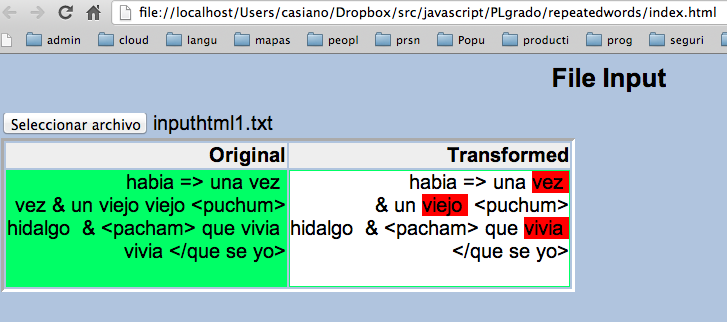
\includegraphics[scale=0.5]{chapter2/repeated_words.png}
\end{center}
\label{figure:csv}
\caption{Ejemplo de pantalla de La aplicación para el Análisis de Datos en Formato CSV}
\end{figure}

\parrafo{Estructura}

\begin{verbatim}
<pre>
[~/Dropbox/src/javascript/PLgrado/repeatedwords(master)]$  tree --charset utf-8 
.
├── README
├── global.css
├── index.html
├── input.txt
├── input2.txt
├── inputhtml1.txt
└── repeated_words.js

0 directories, 7 files
</pre>
\end{verbatim}

\parrafo{index.html}
\begin{verbatim}
[~/Dropbox/src/javascript/PLgrado/repeatedwords(master)]$ cat index.html 
<html>
  <head>
     <meta http-equiv="Content-Type" content="text/html; charset=UTF-8">
     <title>File Input</title>
     <link href="global.css" rel="stylesheet" type="text/css">

     <script type="text/javascript" src="../../underscore/underscore.js"></script>
     <script type="text/javascript" src="../../jquery/starterkit/jquery.js"></script>
     <script type="text/javascript" src="repeated_words.js"></script>
  </head>
  <body>
    <h1>File Input</h1>
    <input type="file" id="fileinput" />
    <div id="out" class="hidden">
    <table>
      <tr><th>Original</th><th>Transformed</th></tr>
      <tr>
        <td>
          <pre class="input" id="initialinput"></pre>
        </td>
        <td>
          <pre class="output" id="finaloutput"></pre>
        </td>
      </tr>
    </table>
    </div>
  </body>
</html>
\end{verbatim}

\begin{enumerate}
\item 
\htmladdnormallink{Tag input}{http://www.w3.org/TR/html-markup/input.file.html}
\end{enumerate}
\parrafo{global.css}

Rellena los estilos para \verb|hidden| y \verb|unhidden|:
\begin{verbatim}
[~/Dropbox/src/javascript/PLgrado/repeatedwords(master)]$ cat global.css 
html *
{
   font-size: large; 
   /* The !important ensures that nothing can override what you've set in this style (unless it is also important). */
   font-family: Arial;
}

.thumb {
    height: 75px;
    border: 1px solid #000;
    margin: 10px 5px 0 0;
  }

h1            { text-align: center; font-size: x-large; }
th, td        { vertical-align: top; text-align: right; }   
/* #finaltable  * { color: white; background-color: black; }   */

/* #finaltable table { border-collapse:collapse; } */
/* #finaltable table, td { border:1px solid white; } */
#finaltable:hover td { background-color: blue; } 
tr:nth-child(odd)    { background-color:#eee; }
tr:nth-child(even)    { background-color:#00FF66; }
input        { text-align: right;  border: none;       }     /* Align input to the right  */
textarea     { border: outset; border-color: white;       }                        
table        { border: inset; border-color: white; }
.hidden      { display: ____; }
.unhidden    { display: _____; }
table.center { margin-left:auto; margin-right:auto; }
#result      { border-color: red; }
tr.error       { background-color: red; }
pre.output   { background-color: white; }
span.repeated { background-color: red }

body
{
 background-color:#b0c4de;  /* blue */
\end{verbatim}

\begin{enumerate}
\item 
\htmladdnormallink{CSS display Property}{http://www.w3schools.com/cssref/pr_class_display.asp}
\item 
\htmladdnormallink{Diferencias entre "Display" y "Visibility"}{http://www.luiscanada.com/manualCSS/css-display-visibility.php}
\end{enumerate}
\parrafo{repeated\_words.js}

Rellena las expresiones regulares que faltan:
\begin{verbatim}
[~/srcPLgrado/repeatedwords(master)]$ cat repeated_words.js 
"use strict"; // Use ECMAScript 5 strict mode in browsers that support it

$(document).ready(function() {
   $("#fileinput").change(calculate);
});

function generateOutput(contents) {
  return contents.replace(/____________________/__,'__________________________________');
}

function calculate(evt) {
  var f = evt.target.files[0]; 
  var contents = '';

  if (f) {
    var r = new FileReader();
    r.onload = function(e) { 
      contents = e.target.result;
      var escaped  = escapeHtml(contents);
      var outdiv = document.getElementById("out");
      outdiv.className = 'unhidden';
      finaloutput.innerHTML = generateOutput(escaped);
      initialinput.innerHTML = escaped;

    }
    r.readAsText(f);
  } else { 
    alert("Failed to load file");
  }
}

var entityMap = {
    "&": "&amp;",
    "<": "&lt;",
    ">": "&gt;",
    '"': '&quot;',
    "'": '&#39;',
    "/": '&#x2F;'
  };

function escapeHtml(string) {
  return String(string).replace(/_________/g, function (s) {
    return ____________;
  });
\end{verbatim}

\begin{enumerate}
\item 
\htmladdnormallink{jQuery event.target}{http://api.jquery.com/event.target/}
\item 
\htmladdnormallink{HTML 5 File API}{http://www.w3.org/TR/FileAPI/}
\item 
\htmladdnormallink{HTML 5 File API: FileReader}{http://www.w3.org/TR/FileAPI/\#dfn-filereader}
\item 
\htmladdnormallink{HTML 5 File API: FileReader}{http://www.w3.org/TR/FileAPI/\#dfn-filereader}
\item 
\htmladdnormallink{element.className}{https://developer.mozilla.org/en-US/docs/DOM/element.className}
\item 
\htmladdnormallink{HTML Entities}{http://www.w3schools.com/html/html_entities.asp}
\item 
\htmladdnormallink{Tutorials:Getting Started with jQuery}{http://docs.jquery.com/Tutorials:Getting_Started_with_jQuery}
\item 
\htmladdnormallink{Underscore: template}{http://underscorejs.org/\#template}
\end{enumerate}

\parrafo{Ficheros de Entrada}
\begin{verbatim}
[~/Dropbox/src/javascript/PLgrado/repeatedwords(master)]$ cat input2.txt 
habia una vez 
vez un viejo viejo
hidalgo que vivia 
vivia
[~/Dropbox/src/javascript/PLgrado/repeatedwords(master)]$ cat input.txt 
one one
nothing rep
is two three
three four
[~/Dropbox/src/javascript/PLgrado/repeatedwords(master)]$ cat inputhtml1.txt 
habia => una vez 
vez & un viejo viejo <puchum>
hidalgo  & <pacham> que vivia 
vivia </que se yo>

\end{verbatim}

\section{Ejercicios}
El formato  \cei{INI} es un formato estandar 
para la escritura de ficheros de configuración. 
Su estrucutra básica se compone de
"secciones" y "propiedades". Véase la entrada de la wikipedia
\wikip{INI}{INI\_file}.
\begin{verbatim}
; last modified 1 April 2001 by John Doe
[owner]
name=John Doe
organization=Acme Widgets Inc.
 
[database]
; use IP address in case network name resolution is not working
server=192.0.2.62     
port=143
file = "payroll.dat"
\end{verbatim}
\begin{enumerate}
\item 
Escriba un programa javascript que obtenga las cabeceras de sección de un fichero 
INI
\item 
Escriba un programa javascript que case con los bloques de un fichero INI (cabecera mas lista de pares \verb|parámetro=valor|)

\item 
Se quieren obtener todos los pares nombre-valor, usando paréntesis con memoria para capturar cada parte.

% Match INI section headers page 472
% Match INI section blocks
% Match INI name-value pairs
% practica: INI configuration files
\item  ¿Que casa con cada paréntesis en esta regexp para los  pares nombre-valor?
\begin{verbatim}
> x = "h     = 4"
> r = /([^=]*)(\s*)=(\s*)(.*)/
> r.exec(x)
>
\end{verbatim}
\end{enumerate}

\section{Ejercicios}

\begin{enumerate}
\item 
Escriba una expresión regular que reconozca las cadenas de doble comillas.
Debe permitir la presencia de comillas y caracteres escapados.
\item 
¿Cual es la salida?
\begin{verbatim}
> "bb".match(/b|bb/)

> "bb".match(/bb|b/)

\end{verbatim}

\end{enumerate}

\sectionpractica{Ficheros INI}


\parrafo{index.html}
\begin{verbatim}
<html>
  <head>
     <meta http-equiv="Content-Type" content="text/html; charset=UTF-8">
     <title>INI files</title>
     <link href="global.css" rel="stylesheet" type="text/css">

     <script type="text/javascript" src="../../underscore/underscore.js"></script>
     <script type="text/javascript" src="../../jquery/starterkit/jquery.js"></script>
     <script type="text/javascript" src="______"></script>
  </head>
  <body>
    <h1>INI files</h1>
    <input type="file" id="_________" />
    <div id="out" class="hidden">
    <table>
      <tr><th>Original</th><th>Tokens</th></tr>
      <tr>
        <td>
          <pre class="input" id="____________"></pre>
        </td>
        <td>
          <pre class="output" id="___________"></pre>
        </td>
      </tr>
    </table>
    </div>
  </body>
</html>
\end{verbatim}

\parrafo{global.css}

\begin{verbatim}
[~/Dropbox/src/javascript/PLgrado/ini(master)]$ cat global.css
html *
{
   font-size: large; 
   /* The !important ensures that nothing can override what you've set in this style (unless it is also important). */
   font-family: Arial;
}

.thumb {
    height: 75px;
    border: 1px solid #000;
    margin: 10px 5px 0 0;
  }

h1            { text-align: center; font-size: x-large; }
th, td        { vertical-align: top; text-align: left; }   
/* #finaltable  * { color: white; background-color: black; }   */

/* #finaltable table { border-collapse:collapse; } */
/* #finaltable table, td { border:1px solid white; } */
#finaltable:hover td { background-color: blue; } 
tr:nth-child(odd)    { background-color:#eee; }
tr:nth-child(even)    { background-color:#00FF66; }
input        { text-align: right;  border: none;       }     /* Align input to the right  */
textarea     { border: outset; border-color: white;       }                        
table        { border: inset; border-color: white; }
.hidden      { display: ____; }
.unhidden    { display: _____; }
table.center { margin-left:auto; margin-right:auto; }
#result      { border-color: red; }
tr.error       { background-color: red; }
pre.output   { background-color: white; }
span.repeated { background-color: red }
span.header { ________________: ____ }
span.comments { ________________: ______ }
span.blanks { ________________: _____ }
span.nameEqualValue { ________________: ____ }
span.error { ________________: ___ }

body
{
 background-color:#b0c4de;  /* blue */
}
\end{verbatim}

\parrafo{Ficheros de Prueba}

\begin{verbatim}
~/Dropbox/src/javascript/PLgrado/ini(master)]$ cat input.ini 
; last modified 1 April 2001 by John Doe
[owner]
name=John Doe
organization=Acme Widgets Inc.

[database]
; use IP address in case network name resolution is not working
server=192.0.2.62     
port=143
file = "payroll.dat"
\end{verbatim}

\begin{verbatim}
$ cat input2.ini 
[special_fields] 
required = "EmailAddr,FirstName,LastName,Mesg" 
csvfile = "contacts.csv" 
csvcolumns = "EmailAddr,FirstName,LastName,Mesg,Date,Time" 

[email_addresses] 
sales = "jack@yahoo.com,mary@my-sales-force.com,president@my-company.com"
\end{verbatim}

\begin{verbatim}
$ cat inputerror.ini
[owner]
name=John Doe
organization$Acme Widgets Inc.
 
[database
; use IP address in case network name resolution is not working
server=192.0.2.62     
port=143
file = "payroll.dat"
\end{verbatim}

\parrafo{ini.js}


\begin{verbatim}
[~/Dropbox/src/javascript/PLgrado/ini(master)]$ cat ini.js 
"use ______"; // Use ECMAScript 5 strict mode in browsers that support it

$(document)._____(function() {
   $("#fileinput").______(calculate);
});

function calculate(evt) {
  var f = evt.target.files[0]; 

  if (f) {
    var r = new __________();
    r.onload = function(e) { 
      var contents = e.target.______;
      
      var tokens = lexer(contents);
      var pretty = tokensToString(tokens);
      
      out.className = 'unhidden';
      initialinput._________ = contents;
      finaloutput._________ = pretty;
    }
    r.__________(f); // Leer como texto
  } else { 
    alert("Failed to load file");
  }
}

var temp = '<li> <span class = "<%= ______ %>"> <%= _ %> </span>\n';

function tokensToString(tokens) {
   var r = '';
   for(var i in tokens) {
     var t = tokens[i];
     var s = JSON.stringify(t, undefined, 2);
     s = _.template(temp, {t: t, s: s});
     r += s;
   }
   return '<ol>\n'+r+'</ol>';
}

function lexer(input) {
  var blanks         = /^___/;
  var iniheader      = /^________________/;
  var comments       = /^________/;
  var nameEqualValue = /^________________________/;
  var any            = /^_______/;

  var out = [];
  var m = null;

  while (input != '') {
    if (m = blanks.____(input)) {
      input = input.substr(m.index+___________);
      out.push({ type : ________, match: _ });
    }
    else if (m = iniheader.exec(input)) {
      input = input.substr(___________________);
      _______________________________________ // avanzemos en input
    }
    else if (m = comments.exec(input)) {
      input = input.substr(___________________);
      _________________________________________
    }
    else if (m = nameEqualValue.exec(input)) {
      input = input.substr(___________________);
      _______________________________________________
    }
    else if (m = any.exec(input)) {
      _______________________________________
      input = '';
    }
    else {
      alert("Fatal Error!"+substr(input,0,20));
      input = '';
    }
  }
  return out;
}
\end{verbatim}

\begin{enumerate}
\item 
\htmladdnormallink{JSON.stringify}{https://developer.mozilla.org/en-US/docs/JavaScript/Reference/Global_Objects/JSON/stringify}
\item 
\htmladdnormallink{www.json.org}{http://www.json.org/}
\item 
\htmladdnormallink{JSON in JavaScript}{http://www.json.org/js.html}
\item 
\htmladdnormallink{Underscore: template}{http://underscorejs.org/\#template}
\item 
\htmladdnormallink{Stackoverflow::how to use Underscore template}{http://stackoverflow.com/questions/4778881/how-to-use-underscore-js-as-a-template-engine}
\end{enumerate}

\sectionpractica{Analizador Léxico para Un Subconjunto de JavaScript}

\begin{enumerate}
\item  Clone el proyecto 
\htmladdnormallink{ull-etsii-grado-pl-minijavascript}{https://github.com/crguezl/ull-etsii-grado-pl-minijavascript} en github. Rellene las partes que faltan en cada fichero.
\end{enumerate}
\section{Definición y Diseño de Lenguajes}
% ver herramientas firefox y chrome para desarrollo



\section{Expresiones Regulares Posix en C}
Las Expresiones Regulares 'a la Perl' no forman parte de ANSI C. 
La forma mas sencilla de usar regexps en C es utilizando la versión POSIX de la
librería que viene con la mayoría de los Unix.
Sigue un ejemplo que usa regex POSIX en C:
\begin{verbatim}
[~/src/C/regexp]$ cat use_posix.c 
#include <stdio.h>
#include <stdlib.h>
#include <regex.h>        

int main() {
       regex_t regex;
       int reti;
       char msgbuf[100];

/* Compile regular expression */
        reti = regcomp(&regex, "^a[[:alnum:]]", 0);
        if( reti ){ fprintf(stderr, "Could not compile regex\n"); exit(1); }

/* Execute regular expression */
        reti = regexec(&regex, "abc", 0, NULL, 0);
        if( !reti ){
                puts("Match");
        }
        else if( reti == REG_NOMATCH ){
                puts("No match");
        }
        else{
                regerror(reti, &regex, msgbuf, sizeof(msgbuf));
                fprintf(stderr, "Regex match failed: %s\n", msgbuf);
                exit(1);
        }

/* Free compiled regular expression if you want to use the regex_t again */
    regfree(&regex);
}
\end{verbatim}
Compilación y ejecución:
\begin{verbatim}
[~/src/C/regexp]$ cc use_posix.c  -o use_posix
[~/src/C/regexp]$ ./use_posix 
Match
\end{verbatim}


\parrafo{Enlaces Relacionados}
\begin{enumerate}
\item 
\htmladdnormallink{Regular Expression Matching in GNU C}{http://www.gnu.org/software/libc/manual/html_node/Regular-Expressions.html}
\item 
\htmladdnormallink{Pattern Matching in GNU C}{http://www.gnu.org/software/libc/manual/html_node/Pattern-Matching.html\#Pattern-Matching}
\item 
\htmladdnormallink{PCRE}{http://www.pcre.org/}
\item 
\htmladdnormallink{PCRE doc}{http://www.pcre.org/pcre.txt}
\end{enumerate}
